% !TeX root = ../../thesis.tex
\chapter{Results and Discussion}

\section{Performance of EOM-CC2 Related Methods}
\ldots
\subsection{Basis Set Dependence of EA-EOM-CC2 in Dipole Bound Anions}
\ldots
\begin{landscape}
\begin{table}[pb!]
  \centering
  \small
  \begin{tabular}{cccccccccccc}
    & & \multicolumn{6}{c}{RI-CC2} & \multicolumn{2}{c}{RI-CCSD} & & \\
    \cmidrule(lr){3-8} \cmidrule(lr){9-10} 
    & & \multicolumn{4}{c}{aug-cc-pVTZ} & pVDZ & pVQZ & pVDZ & pTDZ & & \\
    \multicolumn{2}{c}{Molecule} & 2s1p & 4s2p & 6s3p & 8s4p & 6s3p & 6s3p & 6s3p & 6s3p & KT & \textmu (D) \\
    \hline
    Acetaldehyde & \ce{CH3CHO} & -156.7 & -27.8 & -3.2 & 0.8 & -4.6 & -3.2 & -4.6 & -3.1 & -0.428 & 3.29 \\
    Acetone & \ce{(CH3)2CO} & -114.9 & -16.8 & 1.3 & 3.3 & -0.3 & 0.9 & -0.5 & 0.9 & -5.1 & 3.46 \\
    Acetonitrile & \ce{CH3CN} & -61.2 & 12.6 & 19.9 & 20.1 & 18.2 & 20.3 & 17.1 & 18.4 & 4.2 & 4.29 \\
    Benzaldehyde & \ce{C6H5CHO} & -97.1 & -2.1 & 8.9 & 9.6 & 7.4 & 9.1 & 3.4 & 4.6 & -4.9 & 3.77 \\
    N,N-Dimethylformamide & \ce{(CH3)2NCHO} & -81.1 & 5.4 & 14.1 & 14.4 & 13.2 & 14.4 & 13.3 & 13.7 & 1.9 & 4.48 \\
    DMSO & \ce{(CH3)2SO} & -84.5 & 4.0 & 15.4 & 16.1 & 14.8 & 15.5 & 14.7 & 14.9 & 2.1 & 4.63 \\
    Formamide & \ce{CH3NO} & -92.2 & 1.1 & 16.2 & 17.2 & 15.1 & 17.0 & 15.1 & 15.9 & 3.4 & 4.28 \\
    Methylisocyanide & \ce{CH3NC} & -95.1 & -0.5 & 10.0 & 10.5 & 9.5 & 10.1 & 8.8 & 9.0 & -1.8 & 3.59 \\
    Nitrobenzene & \ce{C6H5NO2} & -63.6 & 30.6 & 34.8 & 34.8 & 32.5 & - & 25.0 & 25.9 & 5.4 & 5.15 \\
    Nitromethane & \ce{CH3NO2} & -82.9 & 5.7 & 14.2 & 14.7 & 13.0 & 14.7 & 12.9 & 13.7 & 3.5 & 4.10 \\
    Nitrosobenzene & \ce{C6H5NO} & -125.0 & 1.0 & 11.4 & - & 9.9 & - & 5.1 & 6.0 & -4.1 & 3.73 \\
    Phenylisocyanide & \ce{C6H5NC} & -82.7 & 8.6 & 16.3 & 16.5 & 15.2 & 16.7 & 9.0 & 9.2 & -4.9 & 3.61 \\
    Pyridazine & \ce{C4H4N2} & -80.7 & 20.5 & 26.3 & 26.4 & 25.0 & 26.7 & 18.6 & 19.1 & 1.7 & 4.41 \\
    Vinylene carbonate & \ce{C3H2O3} & -82.5 & 20.9 & 27.2 & 27.4 & 26.4 & 27.7 & 25.1 & 25.5 & 10 & 5.05 \\
    \cmidrule(lr){2-10} 
    & MAE & 105.3 & 8.8 & 2.8 & 3.4 & 2.3 & 2.4 & 0.8 & ref. & & \\
\end{tabular}
\caption{EOM-EA binding energies of dipole-bound radical anions computed using different augmented Dunning basis sets and RI-CC2 and RI-CCSD for the the test set of moluces \cite{paran2024performance}. A positive value corresponds to a bound electron. Koopmans' theorem (KT), and dipole momment (\textmu), calculated at the HF level, and mean absolute error (MAE) are also given. The values are in meV and D respectively.}
\label{tab:basis}
\end{table}
\end{landscape}


\subsection{Performance of EA-EOM-CC2 on Valence Bound Radical Anion States of Quinones}

\iffalse
\begin{table}[h!]
  \centering
  \begin{tabular}{
    >{\centering\arraybackslash}m{1.1cm}
    >{\centering\arraybackslash}m{0.6cm}
    >{\centering\arraybackslash}m{1.1cm}
    >{\centering\arraybackslash}m{0.6cm}
    >{\centering\arraybackslash}m{0.5cm}
  }
 & \multicolumn{2}{c}{ref. \cite{schulz2018systematic}} & \multicolumn{2}{c}{RI-CC2}  \\
 \cmidrule(lr){2-3} \cmidrule(lr){4-5}
Molecule & Exp (aEA) & CCSD(T) +E\textsubscript{CBS} & No SCS & SCS \\
\hline
1 & 1.91 & 1.64 & 2.02 & 1.54 \\
2 & 1.85 & 1.57 & 1.95 & - \\
3 & 1.76 & 1.49 & 1.89 & 1.39 \\
4 & 1.77 & 1.5 & 1.89 & 1.40 \\
5 & 1.69 & 1.43 & 1.84 & 1.34 \\
6 & 1.62 & 1.42 & 1.83 & 1.32 \\
7 & 1.72 & 1.32 & 1.65 & 1.17 \\
8 & 1.86 & 1.5 & 1.88 & 1.39 \\
9 & 1.81 & 1.55 & 1.97 & - \\
10 & 1.74 & 1.51 & 1.92 & 1.45 \\
\end{tabular}
\caption{Quinones.}
\label{tab:quinones}
\end{table}

\begin{figure}[th!]
  \centering
  % GNUPLOT: LaTeX picture with Postscript
\begingroup
  \makeatletter
  \providecommand\color[2][]{%
    \GenericError{(gnuplot) \space\space\space\@spaces}{%
      Package color not loaded in conjunction with
      terminal option `colourtext'%
    }{See the gnuplot documentation for explanation.%
    }{Either use 'blacktext' in gnuplot or load the package
      color.sty in LaTeX.}%
    \renewcommand\color[2][]{}%
  }%
  \providecommand\includegraphics[2][]{%
    \GenericError{(gnuplot) \space\space\space\@spaces}{%
      Package graphicx or graphics not loaded%
    }{See the gnuplot documentation for explanation.%
    }{The gnuplot epslatex terminal needs graphicx.sty or graphics.sty.}%
    \renewcommand\includegraphics[2][]{}%
  }%
  \providecommand\rotatebox[2]{#2}%
  \@ifundefined{ifGPcolor}{%
    \newif\ifGPcolor
    \GPcolortrue
  }{}%
  \@ifundefined{ifGPblacktext}{%
    \newif\ifGPblacktext
    \GPblacktexttrue
  }{}%
  % define a \g@addto@macro without @ in the name:
  \let\gplgaddtomacro\g@addto@macro
  % define empty templates for all commands taking text:
  \gdef\gplbacktext{}%
  \gdef\gplfronttext{}%
  \makeatother
  \ifGPblacktext
    % no textcolor at all
    \def\colorrgb#1{}%
    \def\colorgray#1{}%
  \else
    % gray or color?
    \ifGPcolor
      \def\colorrgb#1{\color[rgb]{#1}}%
      \def\colorgray#1{\color[gray]{#1}}%
      \expandafter\def\csname LTw\endcsname{\color{white}}%
      \expandafter\def\csname LTb\endcsname{\color{black}}%
      \expandafter\def\csname LTa\endcsname{\color{black}}%
      \expandafter\def\csname LT0\endcsname{\color[rgb]{1,0,0}}%
      \expandafter\def\csname LT1\endcsname{\color[rgb]{0,1,0}}%
      \expandafter\def\csname LT2\endcsname{\color[rgb]{0,0,1}}%
      \expandafter\def\csname LT3\endcsname{\color[rgb]{1,0,1}}%
      \expandafter\def\csname LT4\endcsname{\color[rgb]{0,1,1}}%
      \expandafter\def\csname LT5\endcsname{\color[rgb]{1,1,0}}%
      \expandafter\def\csname LT6\endcsname{\color[rgb]{0,0,0}}%
      \expandafter\def\csname LT7\endcsname{\color[rgb]{1,0.3,0}}%
      \expandafter\def\csname LT8\endcsname{\color[rgb]{0.5,0.5,0.5}}%
    \else
      % gray
      \def\colorrgb#1{\color{black}}%
      \def\colorgray#1{\color[gray]{#1}}%
      \expandafter\def\csname LTw\endcsname{\color{white}}%
      \expandafter\def\csname LTb\endcsname{\color{black}}%
      \expandafter\def\csname LTa\endcsname{\color{black}}%
      \expandafter\def\csname LT0\endcsname{\color{black}}%
      \expandafter\def\csname LT1\endcsname{\color{black}}%
      \expandafter\def\csname LT2\endcsname{\color{black}}%
      \expandafter\def\csname LT3\endcsname{\color{black}}%
      \expandafter\def\csname LT4\endcsname{\color{black}}%
      \expandafter\def\csname LT5\endcsname{\color{black}}%
      \expandafter\def\csname LT6\endcsname{\color{black}}%
      \expandafter\def\csname LT7\endcsname{\color{black}}%
      \expandafter\def\csname LT8\endcsname{\color{black}}%
    \fi
  \fi
    \setlength{\unitlength}{0.0500bp}%
    \ifx\gptboxheight\undefined%
      \newlength{\gptboxheight}%
      \newlength{\gptboxwidth}%
      \newsavebox{\gptboxtext}%
    \fi%
    \setlength{\fboxrule}{0.5pt}%
    \setlength{\fboxsep}{1pt}%
    \definecolor{tbcol}{rgb}{1,1,1}%
\begin{picture}(3660.00,3380.00)%
    \gplgaddtomacro\gplbacktext{%
      \csname LTb\endcsname%%
      \put(616,824){\makebox(0,0)[r]{\strut{}$1.2$}}%
      \csname LTb\endcsname%%
      \put(616,1349){\makebox(0,0)[r]{\strut{}$1.4$}}%
      \csname LTb\endcsname%%
      \put(616,1873){\makebox(0,0)[r]{\strut{}$1.6$}}%
      \csname LTb\endcsname%%
      \put(616,2397){\makebox(0,0)[r]{\strut{}$1.8$}}%
      \csname LTb\endcsname%%
      \put(616,2921){\makebox(0,0)[r]{\strut{}$2$}}%
      \csname LTb\endcsname%%
      \put(714,386){\makebox(0,0){\strut{}$1.3$}}%
      \csname LTb\endcsname%%
      \put(1090,386){\makebox(0,0){\strut{}$1.35$}}%
      \csname LTb\endcsname%%
      \put(1466,386){\makebox(0,0){\strut{}$1.4$}}%
      \csname LTb\endcsname%%
      \put(1842,386){\makebox(0,0){\strut{}$1.45$}}%
      \csname LTb\endcsname%%
      \put(2218,386){\makebox(0,0){\strut{}$1.5$}}%
      \csname LTb\endcsname%%
      \put(2594,386){\makebox(0,0){\strut{}$1.55$}}%
      \csname LTb\endcsname%%
      \put(2970,386){\makebox(0,0){\strut{}$1.6$}}%
      \csname LTb\endcsname%%
      \put(3346,386){\makebox(0,0){\strut{}$1.65$}}%
    }%
    \gplgaddtomacro\gplfronttext{%
      \csname LTb\endcsname%%
      \put(3271,3009){\makebox(0,0){\color{blue}\textbf{1}}}%
      \csname LTb\endcsname%%
      \put(2744,2825){\makebox(0,0){\color{blue}\textbf{2}}}%
      \csname LTb\endcsname%%
      \put(2143,2668){\makebox(0,0){\color{blue}\textbf{3}}}%
      \csname LTb\endcsname%%
      \put(2218,2668){\makebox(0,0){\color{blue}\textbf{4}}}%
      \csname LTb\endcsname%%
      \put(1691,2537){\makebox(0,0){\color{blue}\textbf{5}}}%
      \csname LTb\endcsname%%
      \put(1616,2511){\makebox(0,0){\color{blue}\textbf{6}}}%
      \csname LTb\endcsname%%
      \put(864,2039){\makebox(0,0){\color{blue}\textbf{7}}}%
      \csname LTb\endcsname%%
      \put(2218,2642){\makebox(0,0){\color{blue}\textbf{8}}}%
      \csname LTb\endcsname%%
      \put(2594,2878){\makebox(0,0){\color{blue}\textbf{9}}}%
      \csname LTb\endcsname%%
      \put(2293,2747){\makebox(0,0){\color{blue}\textbf{10}}}%
      \csname LTb\endcsname%%
      \put(3271,1681){\makebox(0,0){\color{red}\textbf{1}}}%
      \csname LTb\endcsname%%
      \put(2143,1287){\makebox(0,0){\color{red}\textbf{3}}}%
      \csname LTb\endcsname%%
      \put(2218,1314){\makebox(0,0){\color{red}\textbf{4}}}%
      \csname LTb\endcsname%%
      \put(1691,1156){\makebox(0,0){\color{red}\textbf{5}}}%
      \csname LTb\endcsname%%
      \put(1616,1104){\makebox(0,0){\color{red}\textbf{6}}}%
      \csname LTb\endcsname%%
      \put(864,711){\makebox(0,0){\color{red}\textbf{7}}}%
      \csname LTb\endcsname%%
      \put(2218,1287){\makebox(0,0){\color{red}\textbf{8}}}%
      \csname LTb\endcsname%%
      \put(2293,1445){\makebox(0,0){\color{red}\textbf{10}}}%
      \csname LTb\endcsname%%
      \put(2590,1072){\makebox(0,0)[r]{\strut{}Ref.}}%
      \csname LTb\endcsname%%
      \put(2590,896){\makebox(0,0)[r]{\strut{}No SCS}}%
      \csname LTb\endcsname%%
      \put(2590,721){\makebox(0,0)[r]{\strut{}SCS}}%
      \csname LTb\endcsname%%
      \put(161,1873){\rotatebox{-270.00}{\makebox(0,0){\strut{}Method Energy (eV)}}}%
      \csname LTb\endcsname%%
      \put(2030,123){\makebox(0,0){\strut{}Reference Energy (eV)}}%
    }%
    \gplbacktext
    \put(0,0){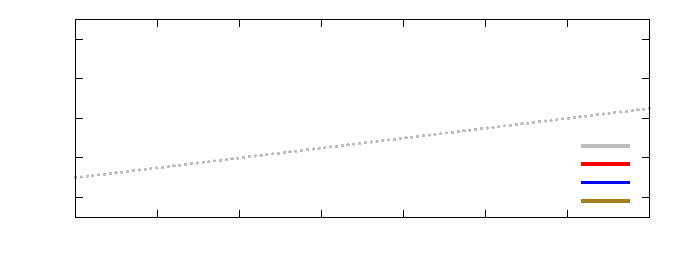
\includegraphics[width={183.00bp},height={169.00bp}]{Quinones}}%
    \gplfronttext
  \end{picture}%
\endgroup

  %figsize is set in image/test.gp 
  \caption[Short caption for Table of Figures]{Favorable Interaction with water.}
  \label{fig:Quinones}
\end{figure}
\fi

\begin{figure}[h!]
  \centering
  \begin{minipage}[t]{0.48\textwidth}
    \centering
    \begin{tabular}{
      >{\centering\arraybackslash}m{0.7cm}
      >{\centering\arraybackslash}m{0.6cm}
      >{\centering\arraybackslash}m{1.1cm}
      >{\centering\arraybackslash}m{0.6cm}
      >{\centering\arraybackslash}m{0.5cm}
    }
   & \multicolumn{2}{c}{Ref. \cite{schulz2018systematic}} & \multicolumn{2}{c}{RI-CC2}  \\
   \cmidrule(lr){2-3} \cmidrule(lr){4-5}
  Mol. & Exp (aEA) & CCSD(T) +E\textsubscript{CBS} & No SCS & SCS \\
  \hline
  1 & 1.91 & 1.64 & 2.02 & 1.54 \\
  2 & 1.85 & 1.57 & 1.95 & - \\
  3 & 1.76 & 1.49 & 1.89 & 1.39 \\
  4 & 1.77 & 1.5 & 1.89 & 1.40 \\
  5 & 1.69 & 1.43 & 1.84 & 1.34 \\
  6 & 1.62 & 1.42 & 1.83 & 1.32 \\
  7 & 1.72 & 1.32 & 1.65 & 1.17 \\
  8 & 1.86 & 1.5 & 1.88 & 1.39 \\
  9 & 1.81 & 1.55 & 1.97 & - \\
  10 & 1.74 & 1.51 & 1.92 & 1.45 \\
    \end{tabular}
  \end{minipage}%
  \hfill
  \begin{minipage}[]{0.48\textwidth}
    \centering
    % GNUPLOT: LaTeX picture with Postscript
\begingroup
  \makeatletter
  \providecommand\color[2][]{%
    \GenericError{(gnuplot) \space\space\space\@spaces}{%
      Package color not loaded in conjunction with
      terminal option `colourtext'%
    }{See the gnuplot documentation for explanation.%
    }{Either use 'blacktext' in gnuplot or load the package
      color.sty in LaTeX.}%
    \renewcommand\color[2][]{}%
  }%
  \providecommand\includegraphics[2][]{%
    \GenericError{(gnuplot) \space\space\space\@spaces}{%
      Package graphicx or graphics not loaded%
    }{See the gnuplot documentation for explanation.%
    }{The gnuplot epslatex terminal needs graphicx.sty or graphics.sty.}%
    \renewcommand\includegraphics[2][]{}%
  }%
  \providecommand\rotatebox[2]{#2}%
  \@ifundefined{ifGPcolor}{%
    \newif\ifGPcolor
    \GPcolortrue
  }{}%
  \@ifundefined{ifGPblacktext}{%
    \newif\ifGPblacktext
    \GPblacktexttrue
  }{}%
  % define a \g@addto@macro without @ in the name:
  \let\gplgaddtomacro\g@addto@macro
  % define empty templates for all commands taking text:
  \gdef\gplbacktext{}%
  \gdef\gplfronttext{}%
  \makeatother
  \ifGPblacktext
    % no textcolor at all
    \def\colorrgb#1{}%
    \def\colorgray#1{}%
  \else
    % gray or color?
    \ifGPcolor
      \def\colorrgb#1{\color[rgb]{#1}}%
      \def\colorgray#1{\color[gray]{#1}}%
      \expandafter\def\csname LTw\endcsname{\color{white}}%
      \expandafter\def\csname LTb\endcsname{\color{black}}%
      \expandafter\def\csname LTa\endcsname{\color{black}}%
      \expandafter\def\csname LT0\endcsname{\color[rgb]{1,0,0}}%
      \expandafter\def\csname LT1\endcsname{\color[rgb]{0,1,0}}%
      \expandafter\def\csname LT2\endcsname{\color[rgb]{0,0,1}}%
      \expandafter\def\csname LT3\endcsname{\color[rgb]{1,0,1}}%
      \expandafter\def\csname LT4\endcsname{\color[rgb]{0,1,1}}%
      \expandafter\def\csname LT5\endcsname{\color[rgb]{1,1,0}}%
      \expandafter\def\csname LT6\endcsname{\color[rgb]{0,0,0}}%
      \expandafter\def\csname LT7\endcsname{\color[rgb]{1,0.3,0}}%
      \expandafter\def\csname LT8\endcsname{\color[rgb]{0.5,0.5,0.5}}%
    \else
      % gray
      \def\colorrgb#1{\color{black}}%
      \def\colorgray#1{\color[gray]{#1}}%
      \expandafter\def\csname LTw\endcsname{\color{white}}%
      \expandafter\def\csname LTb\endcsname{\color{black}}%
      \expandafter\def\csname LTa\endcsname{\color{black}}%
      \expandafter\def\csname LT0\endcsname{\color{black}}%
      \expandafter\def\csname LT1\endcsname{\color{black}}%
      \expandafter\def\csname LT2\endcsname{\color{black}}%
      \expandafter\def\csname LT3\endcsname{\color{black}}%
      \expandafter\def\csname LT4\endcsname{\color{black}}%
      \expandafter\def\csname LT5\endcsname{\color{black}}%
      \expandafter\def\csname LT6\endcsname{\color{black}}%
      \expandafter\def\csname LT7\endcsname{\color{black}}%
      \expandafter\def\csname LT8\endcsname{\color{black}}%
    \fi
  \fi
    \setlength{\unitlength}{0.0500bp}%
    \ifx\gptboxheight\undefined%
      \newlength{\gptboxheight}%
      \newlength{\gptboxwidth}%
      \newsavebox{\gptboxtext}%
    \fi%
    \setlength{\fboxrule}{0.5pt}%
    \setlength{\fboxsep}{1pt}%
    \definecolor{tbcol}{rgb}{1,1,1}%
\begin{picture}(3660.00,3380.00)%
    \gplgaddtomacro\gplbacktext{%
      \csname LTb\endcsname%%
      \put(616,824){\makebox(0,0)[r]{\strut{}$1.2$}}%
      \csname LTb\endcsname%%
      \put(616,1349){\makebox(0,0)[r]{\strut{}$1.4$}}%
      \csname LTb\endcsname%%
      \put(616,1873){\makebox(0,0)[r]{\strut{}$1.6$}}%
      \csname LTb\endcsname%%
      \put(616,2397){\makebox(0,0)[r]{\strut{}$1.8$}}%
      \csname LTb\endcsname%%
      \put(616,2921){\makebox(0,0)[r]{\strut{}$2$}}%
      \csname LTb\endcsname%%
      \put(714,386){\makebox(0,0){\strut{}$1.3$}}%
      \csname LTb\endcsname%%
      \put(1090,386){\makebox(0,0){\strut{}$1.35$}}%
      \csname LTb\endcsname%%
      \put(1466,386){\makebox(0,0){\strut{}$1.4$}}%
      \csname LTb\endcsname%%
      \put(1842,386){\makebox(0,0){\strut{}$1.45$}}%
      \csname LTb\endcsname%%
      \put(2218,386){\makebox(0,0){\strut{}$1.5$}}%
      \csname LTb\endcsname%%
      \put(2594,386){\makebox(0,0){\strut{}$1.55$}}%
      \csname LTb\endcsname%%
      \put(2970,386){\makebox(0,0){\strut{}$1.6$}}%
      \csname LTb\endcsname%%
      \put(3346,386){\makebox(0,0){\strut{}$1.65$}}%
    }%
    \gplgaddtomacro\gplfronttext{%
      \csname LTb\endcsname%%
      \put(3271,3009){\makebox(0,0){\color{blue}\textbf{1}}}%
      \csname LTb\endcsname%%
      \put(2744,2825){\makebox(0,0){\color{blue}\textbf{2}}}%
      \csname LTb\endcsname%%
      \put(2143,2668){\makebox(0,0){\color{blue}\textbf{3}}}%
      \csname LTb\endcsname%%
      \put(2218,2668){\makebox(0,0){\color{blue}\textbf{4}}}%
      \csname LTb\endcsname%%
      \put(1691,2537){\makebox(0,0){\color{blue}\textbf{5}}}%
      \csname LTb\endcsname%%
      \put(1616,2511){\makebox(0,0){\color{blue}\textbf{6}}}%
      \csname LTb\endcsname%%
      \put(864,2039){\makebox(0,0){\color{blue}\textbf{7}}}%
      \csname LTb\endcsname%%
      \put(2218,2642){\makebox(0,0){\color{blue}\textbf{8}}}%
      \csname LTb\endcsname%%
      \put(2594,2878){\makebox(0,0){\color{blue}\textbf{9}}}%
      \csname LTb\endcsname%%
      \put(2293,2747){\makebox(0,0){\color{blue}\textbf{10}}}%
      \csname LTb\endcsname%%
      \put(3271,1681){\makebox(0,0){\color{red}\textbf{1}}}%
      \csname LTb\endcsname%%
      \put(2143,1287){\makebox(0,0){\color{red}\textbf{3}}}%
      \csname LTb\endcsname%%
      \put(2218,1314){\makebox(0,0){\color{red}\textbf{4}}}%
      \csname LTb\endcsname%%
      \put(1691,1156){\makebox(0,0){\color{red}\textbf{5}}}%
      \csname LTb\endcsname%%
      \put(1616,1104){\makebox(0,0){\color{red}\textbf{6}}}%
      \csname LTb\endcsname%%
      \put(864,711){\makebox(0,0){\color{red}\textbf{7}}}%
      \csname LTb\endcsname%%
      \put(2218,1287){\makebox(0,0){\color{red}\textbf{8}}}%
      \csname LTb\endcsname%%
      \put(2293,1445){\makebox(0,0){\color{red}\textbf{10}}}%
      \csname LTb\endcsname%%
      \put(2590,1072){\makebox(0,0)[r]{\strut{}Ref.}}%
      \csname LTb\endcsname%%
      \put(2590,896){\makebox(0,0)[r]{\strut{}No SCS}}%
      \csname LTb\endcsname%%
      \put(2590,721){\makebox(0,0)[r]{\strut{}SCS}}%
      \csname LTb\endcsname%%
      \put(161,1873){\rotatebox{-270.00}{\makebox(0,0){\strut{}Method Energy (eV)}}}%
      \csname LTb\endcsname%%
      \put(2030,123){\makebox(0,0){\strut{}Reference Energy (eV)}}%
    }%
    \gplbacktext
    \put(0,0){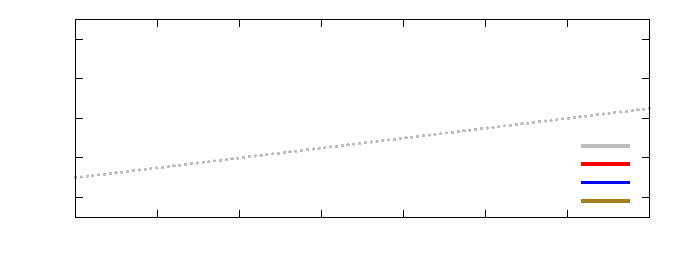
\includegraphics[width={183.00bp},height={169.00bp}]{Quinones}}%
    \gplfronttext
  \end{picture}%
\endgroup

  \end{minipage}
  \refstepcounter{table}\label{tab:quinones}
  \refstepcounter{figure}\label{fig:Quinones}
  \caption*{\textbf{Table~\thetable{}} and \textbf{Figure~\thefigure{}:} Comparison between reference and RI-CC2 data for quinones. The table also includes the experimental value (adiabatic EA instead of veritacl EA).}
  \addcontentsline{lof}{figure}{\protect\numberline{\thefigure}figure valence anion state quinones}
  \addcontentsline{lot}{table}{\protect\numberline{\thetable} table valence anion state quinones}
\end{figure}

SCS improves the result for valence state of CC2, whihc is in accordance with the conclusions from \cite{paran2024performance}. Something to note is that when comparing the results with experiments, one can think that CC2 gets close than CCSD. This however, can be explained by the fact that the experiment measures the adiabatic electron binding energy, while the calculations are performed for the vertical EA. As the former energy 
\ldots
\subsection{Photoelectron Cross-section Calculations from EOM-CC2/CCSD}

\ldots
\section{Study on the Anion States of Ubiquinone}

\ldots
\subsection{Energy and Dipole Surfaces of CoQ}

\ldots
\subsubsection{Q0}
a

\begin{figure}[h!]
  \centering
  \begin{minipage}[]{0.49\textwidth}
    \centering
    \small
    % GNUPLOT: LaTeX picture with Postscript
\begingroup
  \makeatletter
  \providecommand\color[2][]{%
    \GenericError{(gnuplot) \space\space\space\@spaces}{%
      Package color not loaded in conjunction with
      terminal option `colourtext'%
    }{See the gnuplot documentation for explanation.%
    }{Either use 'blacktext' in gnuplot or load the package
      color.sty in LaTeX.}%
    \renewcommand\color[2][]{}%
  }%
  \providecommand\includegraphics[2][]{%
    \GenericError{(gnuplot) \space\space\space\@spaces}{%
      Package graphicx or graphics not loaded%
    }{See the gnuplot documentation for explanation.%
    }{The gnuplot epslatex terminal needs graphicx.sty or graphics.sty.}%
    \renewcommand\includegraphics[2][]{}%
  }%
  \providecommand\rotatebox[2]{#2}%
  \@ifundefined{ifGPcolor}{%
    \newif\ifGPcolor
    \GPcolortrue
  }{}%
  \@ifundefined{ifGPblacktext}{%
    \newif\ifGPblacktext
    \GPblacktexttrue
  }{}%
  % define a \g@addto@macro without @ in the name:
  \let\gplgaddtomacro\g@addto@macro
  % define empty templates for all commands taking text:
  \gdef\gplbacktext{}%
  \gdef\gplfronttext{}%
  \makeatother
  \ifGPblacktext
    % no textcolor at all
    \def\colorrgb#1{}%
    \def\colorgray#1{}%
  \else
    % gray or color?
    \ifGPcolor
      \def\colorrgb#1{\color[rgb]{#1}}%
      \def\colorgray#1{\color[gray]{#1}}%
      \expandafter\def\csname LTw\endcsname{\color{white}}%
      \expandafter\def\csname LTb\endcsname{\color{black}}%
      \expandafter\def\csname LTa\endcsname{\color{black}}%
      \expandafter\def\csname LT0\endcsname{\color[rgb]{1,0,0}}%
      \expandafter\def\csname LT1\endcsname{\color[rgb]{0,1,0}}%
      \expandafter\def\csname LT2\endcsname{\color[rgb]{0,0,1}}%
      \expandafter\def\csname LT3\endcsname{\color[rgb]{1,0,1}}%
      \expandafter\def\csname LT4\endcsname{\color[rgb]{0,1,1}}%
      \expandafter\def\csname LT5\endcsname{\color[rgb]{1,1,0}}%
      \expandafter\def\csname LT6\endcsname{\color[rgb]{0,0,0}}%
      \expandafter\def\csname LT7\endcsname{\color[rgb]{1,0.3,0}}%
      \expandafter\def\csname LT8\endcsname{\color[rgb]{0.5,0.5,0.5}}%
    \else
      % gray
      \def\colorrgb#1{\color{black}}%
      \def\colorgray#1{\color[gray]{#1}}%
      \expandafter\def\csname LTw\endcsname{\color{white}}%
      \expandafter\def\csname LTb\endcsname{\color{black}}%
      \expandafter\def\csname LTa\endcsname{\color{black}}%
      \expandafter\def\csname LT0\endcsname{\color{black}}%
      \expandafter\def\csname LT1\endcsname{\color{black}}%
      \expandafter\def\csname LT2\endcsname{\color{black}}%
      \expandafter\def\csname LT3\endcsname{\color{black}}%
      \expandafter\def\csname LT4\endcsname{\color{black}}%
      \expandafter\def\csname LT5\endcsname{\color{black}}%
      \expandafter\def\csname LT6\endcsname{\color{black}}%
      \expandafter\def\csname LT7\endcsname{\color{black}}%
      \expandafter\def\csname LT8\endcsname{\color{black}}%
    \fi
  \fi
    \setlength{\unitlength}{0.0500bp}%
    \ifx\gptboxheight\undefined%
      \newlength{\gptboxheight}%
      \newlength{\gptboxwidth}%
      \newsavebox{\gptboxtext}%
    \fi%
    \setlength{\fboxrule}{0.5pt}%
    \setlength{\fboxsep}{1pt}%
    \definecolor{tbcol}{rgb}{1,1,1}%
\begin{picture}(3680.00,3680.00)%
    \gplgaddtomacro\gplbacktext{%
      \csname LTb\endcsname%%
      \put(714,959){\makebox(0,0)[r]{\strut{}$-150$}}%
      \csname LTb\endcsname%%
      \put(714,1314){\makebox(0,0)[r]{\strut{}$-100$}}%
      \csname LTb\endcsname%%
      \put(714,1668){\makebox(0,0)[r]{\strut{}$-50$}}%
      \csname LTb\endcsname%%
      \put(714,2023){\makebox(0,0)[r]{\strut{}$0$}}%
      \csname LTb\endcsname%%
      \put(714,2378){\makebox(0,0)[r]{\strut{}$50$}}%
      \csname LTb\endcsname%%
      \put(714,2732){\makebox(0,0)[r]{\strut{}$100$}}%
      \csname LTb\endcsname%%
      \put(714,3087){\makebox(0,0)[r]{\strut{}$150$}}%
      \csname LTb\endcsname%%
      \put(812,570){\makebox(0,0){\strut{}$-180$}}%
      \csname LTb\endcsname%%
      \put(1237,570){\makebox(0,0){\strut{}$-120$}}%
      \csname LTb\endcsname%%
      \put(1663,570){\makebox(0,0){\strut{}$-60$}}%
      \csname LTb\endcsname%%
      \put(2089,570){\makebox(0,0){\strut{}$0$}}%
      \csname LTb\endcsname%%
      \put(2514,570){\makebox(0,0){\strut{}$60$}}%
      \csname LTb\endcsname%%
      \put(2940,570){\makebox(0,0){\strut{}$120$}}%
      \csname LTb\endcsname%%
      \put(3366,570){\makebox(0,0){\strut{}$180$}}%
    }%
    \gplgaddtomacro\gplfronttext{%
      \csname LTb\endcsname%%
      \put(357,2023){\rotatebox{-270.00}{\makebox(0,0){\normalsize $\Psi$}}}%
      \csname LTb\endcsname%%
      \put(2089,306){\makebox(0,0){\normalsize $\Phi$}}%
      \csname LTb\endcsname%%
      \put(1770,2270){\rotatebox{-65.00}{\makebox(0,0){\strut{}\textcolor{black}{\footnotesize 500}}}}%
      \csname LTb\endcsname%%
      \put(2378,2036){\rotatebox{127.00}{\makebox(0,0){\strut{}\textcolor{black}{\footnotesize 400}}}}%
      \csname LTb\endcsname%%
      \put(1783,1948){\rotatebox{-45.00}{\makebox(0,0){\strut{}\textcolor{black}{\footnotesize 400}}}}%
      \csname LTb\endcsname%%
      \put(2029,2484){\rotatebox{152.00}{\makebox(0,0){\strut{}\textcolor{black}{\footnotesize 300}}}}%
      \csname LTb\endcsname%%
      \put(1885,1759){\rotatebox{-38.00}{\makebox(0,0){\strut{}\textcolor{black}{\footnotesize 300}}}}%
      \csname LTb\endcsname%%
      \put(2670,1883){\rotatebox{110.00}{\makebox(0,0){\strut{}\textcolor{black}{\footnotesize 200}}}}%
      \csname LTb\endcsname%%
      \put(1477,2794){\rotatebox{-167.00}{\makebox(0,0){\strut{}\textcolor{black}{\footnotesize 200}}}}%
      \csname LTb\endcsname%%
      \put(2014,1527){\rotatebox{-32.00}{\makebox(0,0){\strut{}\textcolor{black}{\footnotesize 200}}}}%
      \csname LTb\endcsname%%
      \put(1196,2849){\rotatebox{33.00}{\makebox(0,0){\strut{}\textcolor{black}{\footnotesize 100}}}}%
      \csname LTb\endcsname%%
      \put(2481,2849){\rotatebox{51.00}{\makebox(0,0){\strut{}\textcolor{black}{\footnotesize 100}}}}%
      \csname LTb\endcsname%%
      \put(2699,2098){\rotatebox{-73.00}{\makebox(0,0){\strut{}\textcolor{black}{\footnotesize 100}}}}%
      \csname LTb\endcsname%%
      \put(1241,2426){\rotatebox{-30.00}{\makebox(0,0){\strut{}\textcolor{black}{\footnotesize 100}}}}%
      \csname LTb\endcsname%%
      \put(1284,1230){\rotatebox{-38.00}{\makebox(0,0){\strut{}\textcolor{black}{\footnotesize 100}}}}%
      \csname LTb\endcsname%%
      \put(2572,1068){\rotatebox{-46.00}{\makebox(0,0){\strut{}\textcolor{black}{\footnotesize 100}}}}%
      \csname LTb\endcsname%%
      \put(962,2336){\rotatebox{-155.00}{\makebox(0,0){\strut{}\textcolor{black}{\footnotesize 50}}}}%
      \csname LTb\endcsname%%
      \put(2958,2287){\rotatebox{-162.00}{\makebox(0,0){\strut{}\textcolor{black}{\footnotesize 50}}}}%
      \csname LTb\endcsname%%
      \put(1820,2873){\rotatebox{-46.00}{\makebox(0,0){\strut{}\textcolor{black}{\footnotesize 50}}}}%
      \csname LTb\endcsname%%
      \put(1885,1197){\rotatebox{49.00}{\makebox(0,0){\strut{}\textcolor{black}{\footnotesize 50}}}}%
    }%
    \gplbacktext
    \put(0,0){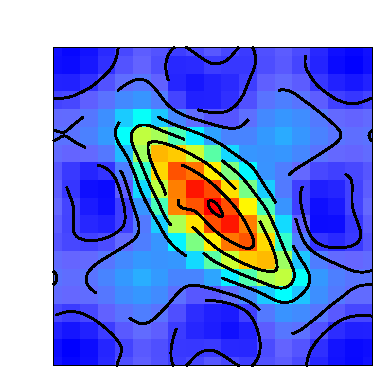
\includegraphics[width={184.00bp},height={184.00bp}]{Figs/Q0_E}}%
    \gplfronttext
  \end{picture}%
\endgroup

  \end{minipage}%
  \hfill
  \begin{minipage}[]{0.47\textwidth}
    \centering
    \small
    % GNUPLOT: LaTeX picture with Postscript
\begingroup
  \makeatletter
  \providecommand\color[2][]{%
    \GenericError{(gnuplot) \space\space\space\@spaces}{%
      Package color not loaded in conjunction with
      terminal option `colourtext'%
    }{See the gnuplot documentation for explanation.%
    }{Either use 'blacktext' in gnuplot or load the package
      color.sty in LaTeX.}%
    \renewcommand\color[2][]{}%
  }%
  \providecommand\includegraphics[2][]{%
    \GenericError{(gnuplot) \space\space\space\@spaces}{%
      Package graphicx or graphics not loaded%
    }{See the gnuplot documentation for explanation.%
    }{The gnuplot epslatex terminal needs graphicx.sty or graphics.sty.}%
    \renewcommand\includegraphics[2][]{}%
  }%
  \providecommand\rotatebox[2]{#2}%
  \@ifundefined{ifGPcolor}{%
    \newif\ifGPcolor
    \GPcolortrue
  }{}%
  \@ifundefined{ifGPblacktext}{%
    \newif\ifGPblacktext
    \GPblacktexttrue
  }{}%
  % define a \g@addto@macro without @ in the name:
  \let\gplgaddtomacro\g@addto@macro
  % define empty templates for all commands taking text:
  \gdef\gplbacktext{}%
  \gdef\gplfronttext{}%
  \makeatother
  \ifGPblacktext
    % no textcolor at all
    \def\colorrgb#1{}%
    \def\colorgray#1{}%
  \else
    % gray or color?
    \ifGPcolor
      \def\colorrgb#1{\color[rgb]{#1}}%
      \def\colorgray#1{\color[gray]{#1}}%
      \expandafter\def\csname LTw\endcsname{\color{white}}%
      \expandafter\def\csname LTb\endcsname{\color{black}}%
      \expandafter\def\csname LTa\endcsname{\color{black}}%
      \expandafter\def\csname LT0\endcsname{\color[rgb]{1,0,0}}%
      \expandafter\def\csname LT1\endcsname{\color[rgb]{0,1,0}}%
      \expandafter\def\csname LT2\endcsname{\color[rgb]{0,0,1}}%
      \expandafter\def\csname LT3\endcsname{\color[rgb]{1,0,1}}%
      \expandafter\def\csname LT4\endcsname{\color[rgb]{0,1,1}}%
      \expandafter\def\csname LT5\endcsname{\color[rgb]{1,1,0}}%
      \expandafter\def\csname LT6\endcsname{\color[rgb]{0,0,0}}%
      \expandafter\def\csname LT7\endcsname{\color[rgb]{1,0.3,0}}%
      \expandafter\def\csname LT8\endcsname{\color[rgb]{0.5,0.5,0.5}}%
    \else
      % gray
      \def\colorrgb#1{\color{black}}%
      \def\colorgray#1{\color[gray]{#1}}%
      \expandafter\def\csname LTw\endcsname{\color{white}}%
      \expandafter\def\csname LTb\endcsname{\color{black}}%
      \expandafter\def\csname LTa\endcsname{\color{black}}%
      \expandafter\def\csname LT0\endcsname{\color{black}}%
      \expandafter\def\csname LT1\endcsname{\color{black}}%
      \expandafter\def\csname LT2\endcsname{\color{black}}%
      \expandafter\def\csname LT3\endcsname{\color{black}}%
      \expandafter\def\csname LT4\endcsname{\color{black}}%
      \expandafter\def\csname LT5\endcsname{\color{black}}%
      \expandafter\def\csname LT6\endcsname{\color{black}}%
      \expandafter\def\csname LT7\endcsname{\color{black}}%
      \expandafter\def\csname LT8\endcsname{\color{black}}%
    \fi
  \fi
    \setlength{\unitlength}{0.0500bp}%
    \ifx\gptboxheight\undefined%
      \newlength{\gptboxheight}%
      \newlength{\gptboxwidth}%
      \newsavebox{\gptboxtext}%
    \fi%
    \setlength{\fboxrule}{0.5pt}%
    \setlength{\fboxsep}{1pt}%
    \definecolor{tbcol}{rgb}{1,1,1}%
\begin{picture}(6180.00,4460.00)%
    \gplgaddtomacro\gplbacktext{%
      \csname LTb\endcsname%%
      \put(1065,841){\makebox(0,0)[r]{\strut{}$-150$}}%
      \csname LTb\endcsname%%
      \put(1065,1307){\makebox(0,0)[r]{\strut{}$-100$}}%
      \csname LTb\endcsname%%
      \put(1065,1772){\makebox(0,0)[r]{\strut{}$-50$}}%
      \csname LTb\endcsname%%
      \put(1065,2237){\makebox(0,0)[r]{\strut{}$0$}}%
      \csname LTb\endcsname%%
      \put(1065,2702){\makebox(0,0)[r]{\strut{}$50$}}%
      \csname LTb\endcsname%%
      \put(1065,3167){\makebox(0,0)[r]{\strut{}$100$}}%
      \csname LTb\endcsname%%
      \put(1065,3633){\makebox(0,0)[r]{\strut{}$150$}}%
      \csname LTb\endcsname%%
      \put(1442,386){\makebox(0,0){\strut{}$-150$}}%
      \csname LTb\endcsname%%
      \put(1907,386){\makebox(0,0){\strut{}$-100$}}%
      \csname LTb\endcsname%%
      \put(2372,386){\makebox(0,0){\strut{}$-50$}}%
      \csname LTb\endcsname%%
      \put(2838,386){\makebox(0,0){\strut{}$0$}}%
      \csname LTb\endcsname%%
      \put(3303,386){\makebox(0,0){\strut{}$50$}}%
      \csname LTb\endcsname%%
      \put(3768,386){\makebox(0,0){\strut{}$100$}}%
      \csname LTb\endcsname%%
      \put(4233,386){\makebox(0,0){\strut{}$150$}}%
    }%
    \gplgaddtomacro\gplfronttext{%
      \csname LTb\endcsname%%
      \put(2838,123){\makebox(0,0){\strut{}$\Phi$}}%
      \csname LTb\endcsname%%
      \put(4861,562){\makebox(0,0)[l]{\strut{}$0$}}%
      \csname LTb\endcsname%%
      \put(4861,1041){\makebox(0,0)[l]{\strut{}$0.5$}}%
      \csname LTb\endcsname%%
      \put(4861,1519){\makebox(0,0)[l]{\strut{}$1$}}%
      \csname LTb\endcsname%%
      \put(4861,1998){\makebox(0,0)[l]{\strut{}$1.5$}}%
      \csname LTb\endcsname%%
      \put(4861,2476){\makebox(0,0)[l]{\strut{}$2$}}%
      \csname LTb\endcsname%%
      \put(4861,2955){\makebox(0,0)[l]{\strut{}$2.5$}}%
      \csname LTb\endcsname%%
      \put(4861,3433){\makebox(0,0)[l]{\strut{}$3$}}%
      \csname LTb\endcsname%%
      \put(4861,3912){\makebox(0,0)[l]{\strut{}$3.5$}}%
      \csname LTb\endcsname%%
      \put(1348,3308){\rotatebox{18.00}{\makebox(0,0){\small 2.70}}}%
      \csname LTb\endcsname%%
      \put(1466,2373){\rotatebox{-131.00}{\makebox(0,0){\small 2.70}}}%
      \csname LTb\endcsname%%
      \put(4361,3027){\rotatebox{-120.00}{\makebox(0,0){\small 2.70}}}%
      \csname LTb\endcsname%%
      \put(3990,1831){\rotatebox{-124.00}{\makebox(0,0){\small 2.70}}}%
      \csname LTb\endcsname%%
      \put(2139,3784){\rotatebox{1.00}{\makebox(0,0){\small 2.21}}}%
      \csname LTb\endcsname%%
      \put(2593,2833){\rotatebox{-29.00}{\makebox(0,0){\small 2.21}}}%
      \csname LTb\endcsname%%
      \put(3351,1938){\rotatebox{-63.00}{\makebox(0,0){\small 2.21}}}%
      \csname LTb\endcsname%%
      \put(4089,2346){\rotatebox{62.00}{\makebox(0,0){\small 2.21}}}%
      \csname LTb\endcsname%%
      \put(1550,2043){\rotatebox{73.00}{\makebox(0,0){\small 2.21}}}%
      \csname LTb\endcsname%%
      \put(2274,2647){\rotatebox{-55.00}{\makebox(0,0){\small 2.21}}}%
      \csname LTb\endcsname%%
      \put(2981,1705){\rotatebox{-29.00}{\makebox(0,0){\small 2.21}}}%
      \csname LTb\endcsname%%
      \put(3435,699){\rotatebox{-16.00}{\makebox(0,0){\small 2.21}}}%
      \csname LTb\endcsname%%
      \put(1695,1656){\rotatebox{83.00}{\makebox(0,0){\small 1.72}}}%
      \csname LTb\endcsname%%
      \put(2459,2104){\rotatebox{-61.00}{\makebox(0,0){\small 1.72}}}%
      \csname LTb\endcsname%%
      \put(2895,1017){\rotatebox{-103.00}{\makebox(0,0){\small 1.72}}}%
      \csname LTb\endcsname%%
      \put(2878,3642){\rotatebox{-129.00}{\makebox(0,0){\small 1.72}}}%
      \csname LTb\endcsname%%
      \put(3142,2565){\rotatebox{-54.00}{\makebox(0,0){\small 1.72}}}%
      \csname LTb\endcsname%%
      \put(3952,2582){\rotatebox{74.00}{\makebox(0,0){\small 1.72}}}%
      \csname LTb\endcsname%%
      \put(1264,904){\rotatebox{32.00}{\makebox(0,0){\small 1.24}}}%
      \csname LTb\endcsname%%
      \put(1971,1846){\rotatebox{41.00}{\makebox(0,0){\small 1.24}}}%
      \csname LTb\endcsname%%
      \put(2631,1050){\rotatebox{-112.00}{\makebox(0,0){\small 1.24}}}%
      \csname LTb\endcsname%%
      \put(3958,3828){\rotatebox{-142.00}{\makebox(0,0){\small 1.24}}}%
      \csname LTb\endcsname%%
      \put(3026,3154){\rotatebox{-73.00}{\makebox(0,0){\small 1.24}}}%
      \csname LTb\endcsname%%
      \put(3805,2822){\rotatebox{73.00}{\makebox(0,0){\small 1.24}}}%
      \csname LTb\endcsname%%
      \put(1701,1109){\rotatebox{49.00}{\makebox(0,0){\small 0.75}}}%
      \csname LTb\endcsname%%
      \put(2344,1084){\rotatebox{-146.00}{\makebox(0,0){\small 0.75}}}%
      \csname LTb\endcsname%%
      \put(3723,3525){\rotatebox{-158.00}{\makebox(0,0){\small 0.75}}}%
      \csname LTb\endcsname%%
      \put(3738,3076){\rotatebox{54.00}{\makebox(0,0){\small 0.75}}}%
      \csname LTb\endcsname%%
      \put(2838,4176){\makebox(0,0){\strut{}Dipole field (Debye)}}%
    }%
    \gplbacktext
    \put(0,0){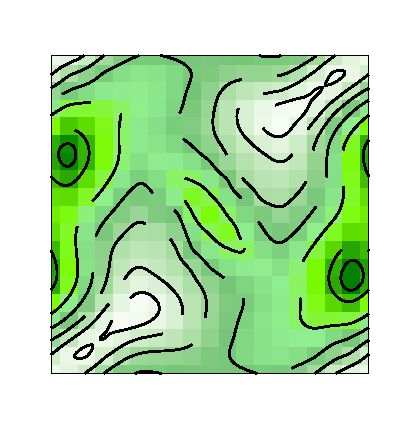
\includegraphics[width={309.00bp},height={223.00bp}]{Q0_d}}%
    \gplfronttext
  \end{picture}%
\endgroup

  \end{minipage}
  \label{fig:Q0_surf}
  \caption[Surfaces of Q0]{Surfaces of Q0. Left: Energy surface. Right: Dipole moment surface.}
\end{figure}

\ldots
\subsubsection{Q1}

\ldots
\subsection{A Simple Cluster Model}
\ldots

\subsection{Interaction with Water}
\ldots
\begin{figure}[th!]
    \centering
    % GNUPLOT: LaTeX picture with Postscript
\begingroup
  \makeatletter
  \providecommand\color[2][]{%
    \GenericError{(gnuplot) \space\space\space\@spaces}{%
      Package color not loaded in conjunction with
      terminal option `colourtext'%
    }{See the gnuplot documentation for explanation.%
    }{Either use 'blacktext' in gnuplot or load the package
      color.sty in LaTeX.}%
    \renewcommand\color[2][]{}%
  }%
  \providecommand\includegraphics[2][]{%
    \GenericError{(gnuplot) \space\space\space\@spaces}{%
      Package graphicx or graphics not loaded%
    }{See the gnuplot documentation for explanation.%
    }{The gnuplot epslatex terminal needs graphicx.sty or graphics.sty.}%
    \renewcommand\includegraphics[2][]{}%
  }%
  \providecommand\rotatebox[2]{#2}%
  \@ifundefined{ifGPcolor}{%
    \newif\ifGPcolor
    \GPcolortrue
  }{}%
  \@ifundefined{ifGPblacktext}{%
    \newif\ifGPblacktext
    \GPblacktexttrue
  }{}%
  % define a \g@addto@macro without @ in the name:
  \let\gplgaddtomacro\g@addto@macro
  % define empty templates for all commands taking text:
  \gdef\gplbacktext{}%
  \gdef\gplfronttext{}%
  \makeatother
  \ifGPblacktext
    % no textcolor at all
    \def\colorrgb#1{}%
    \def\colorgray#1{}%
  \else
    % gray or color?
    \ifGPcolor
      \def\colorrgb#1{\color[rgb]{#1}}%
      \def\colorgray#1{\color[gray]{#1}}%
      \expandafter\def\csname LTw\endcsname{\color{white}}%
      \expandafter\def\csname LTb\endcsname{\color{black}}%
      \expandafter\def\csname LTa\endcsname{\color{black}}%
      \expandafter\def\csname LT0\endcsname{\color[rgb]{1,0,0}}%
      \expandafter\def\csname LT1\endcsname{\color[rgb]{0,1,0}}%
      \expandafter\def\csname LT2\endcsname{\color[rgb]{0,0,1}}%
      \expandafter\def\csname LT3\endcsname{\color[rgb]{1,0,1}}%
      \expandafter\def\csname LT4\endcsname{\color[rgb]{0,1,1}}%
      \expandafter\def\csname LT5\endcsname{\color[rgb]{1,1,0}}%
      \expandafter\def\csname LT6\endcsname{\color[rgb]{0,0,0}}%
      \expandafter\def\csname LT7\endcsname{\color[rgb]{1,0.3,0}}%
      \expandafter\def\csname LT8\endcsname{\color[rgb]{0.5,0.5,0.5}}%
    \else
      % gray
      \def\colorrgb#1{\color{black}}%
      \def\colorgray#1{\color[gray]{#1}}%
      \expandafter\def\csname LTw\endcsname{\color{white}}%
      \expandafter\def\csname LTb\endcsname{\color{black}}%
      \expandafter\def\csname LTa\endcsname{\color{black}}%
      \expandafter\def\csname LT0\endcsname{\color{black}}%
      \expandafter\def\csname LT1\endcsname{\color{black}}%
      \expandafter\def\csname LT2\endcsname{\color{black}}%
      \expandafter\def\csname LT3\endcsname{\color{black}}%
      \expandafter\def\csname LT4\endcsname{\color{black}}%
      \expandafter\def\csname LT5\endcsname{\color{black}}%
      \expandafter\def\csname LT6\endcsname{\color{black}}%
      \expandafter\def\csname LT7\endcsname{\color{black}}%
      \expandafter\def\csname LT8\endcsname{\color{black}}%
    \fi
  \fi
    \setlength{\unitlength}{0.0500bp}%
    \ifx\gptboxheight\undefined%
      \newlength{\gptboxheight}%
      \newlength{\gptboxwidth}%
      \newsavebox{\gptboxtext}%
    \fi%
    \setlength{\fboxrule}{0.5pt}%
    \setlength{\fboxsep}{1pt}%
    \definecolor{tbcol}{rgb}{1,1,1}%
\begin{picture}(7200.00,2880.00)%
    \gplgaddtomacro\gplbacktext{%
      \csname LTb\endcsname%%
      \put(714,562){\makebox(0,0)[r]{\strut{}$-100$}}%
      \csname LTb\endcsname%%
      \put(714,948){\makebox(0,0)[r]{\strut{}$-80$}}%
      \csname LTb\endcsname%%
      \put(714,1334){\makebox(0,0)[r]{\strut{}$-60$}}%
      \csname LTb\endcsname%%
      \put(714,1719){\makebox(0,0)[r]{\strut{}$-40$}}%
      \csname LTb\endcsname%%
      \put(714,2105){\makebox(0,0)[r]{\strut{}$-20$}}%
      \csname LTb\endcsname%%
      \put(714,2491){\makebox(0,0)[r]{\strut{}$0$}}%
      \csname LTb\endcsname%%
      \put(812,386){\makebox(0,0){\strut{}$0$}}%
      \csname LTb\endcsname%%
      \put(1571,386){\makebox(0,0){\strut{}$5$}}%
      \csname LTb\endcsname%%
      \put(2330,386){\makebox(0,0){\strut{}$10$}}%
      \csname LTb\endcsname%%
      \put(3090,386){\makebox(0,0){\strut{}$15$}}%
      \csname LTb\endcsname%%
      \put(3849,386){\makebox(0,0){\strut{}$20$}}%
      \csname LTb\endcsname%%
      \put(4608,386){\makebox(0,0){\strut{}$25$}}%
      \csname LTb\endcsname%%
      \put(5367,386){\makebox(0,0){\strut{}$30$}}%
      \csname LTb\endcsname%%
      \put(6127,386){\makebox(0,0){\strut{}$35$}}%
      \csname LTb\endcsname%%
      \put(6886,386){\makebox(0,0){\strut{}$40$}}%
    }%
    \gplgaddtomacro\gplfronttext{%
      \csname LTb\endcsname%%
      \put(6130,1072){\makebox(0,0)[r]{\strut{}Interaction E}}%
      \csname LTb\endcsname%%
      \put(6130,896){\makebox(0,0)[r]{\strut{}VBA}}%
      \csname LTb\endcsname%%
      \put(6130,721){\makebox(0,0)[r]{\strut{}DBA}}%
      \csname LTb\endcsname%%
      \put(161,1623){\rotatebox{-270.00}{\makebox(0,0){\strut{}Energy (eV)}}}%
      \csname LTb\endcsname%%
      \put(3849,123){\makebox(0,0){\strut{}Distance (\r{A})}}%
    }%
    \gplbacktext
    \put(0,0){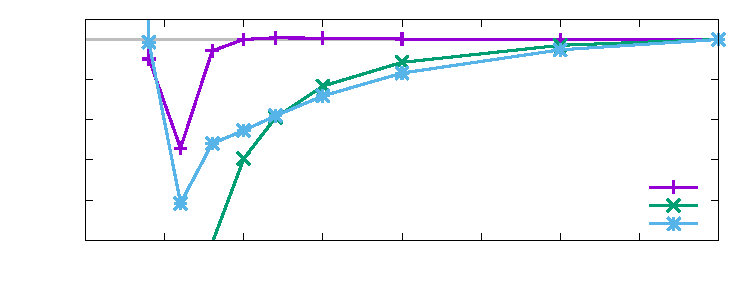
\includegraphics[width={360.00bp},height={144.00bp}]{H2O_fav}}%
    \gplfronttext
  \end{picture}%
\endgroup

    %figsize is set in image/test.gp 
    \caption[Short caption for Table of Figures]{Favorable Interaction with water.}
    \label{fig:H2O_fav}
\end{figure}

\subsection{Effect of Nearby Amionacids}
\ldots

\subsubsection{Serine}
\ldots
\subsubsection{Threonine}
\ldots
\subsubsection{Apsaragine}
\ldots
\subsubsection{Isoleucine}
\ldots

%%%%%%%%%%%%%%%%%%%%%%%%%%%%%%%%%%%%%%%%%%%%%%%%%%
% Keep the following \cleardoublepage at the end of this file, 
% otherwise \includeonly includes empty pages.
\cleardoublepage

% vim: tw=70 nocindent expandtab foldmethod=marker foldmarker={{{}{,}{}}}